\documentclass{beamer}

\usepackage{handoutWithNotes}
\pgfpagesuselayout{4 on 1 with notes}[a4paper,border shrink=5mm]

\usetheme{default}
\beamertemplatenavigationsymbolsempty

%http://mikedewar.wordpress.com/2009/02/25/latex-beamer-python-beauty/
%\definecolor{fore}{RGB}{249,242,215}
\definecolor{fore}{RGB}{51,51,51}
%{249,242,215}
%\definecolor{back}{RGB}{51,51,51}
\definecolor{back}{RGB}{249,242,215}
%{RGB}{51,51,51}
\definecolor{title}{RGB}{230,96,6}
%{255,0,90}
%http://meyerweb.com/eric/tools/color-blend/
%http://www.census.gov/population/international/data/worldpop/table_population.php
\setbeamercolor{titlelike}{fg=title}
\setbeamercolor{normal text}{fg=fore,bg=back}

\useinnertheme{rectangles}
\definecolor{UniBlue}{RGB}{34,139,34}
\setbeamercolor*{item}{fg=UniBlue}

\usepackage{colortbl}
\usepackage{caption}
\usepackage{listings,bera}
\usepackage{lipsum}
\newcommand\Fontvi{\fontsize{6}{7.2}\selectfont}
\newcommand\Fontvii{\fontsize{7}{7.5}\selectfont}
\newcommand\Fontviii{\fontsize{8}{7.8}\selectfont}
\newcommand\Fontix{\fontsize{9}{8.3}\selectfont}
\definecolor{keywords}{RGB}{255,102,0}
%{255,0,90}
\definecolor{comments}{RGB}{51,153,204}
%\definecolor{comments}{RGB}{83,121,170}
\setbeamertemplate{caption}[numbered]
%\useoutertheme{infolines}
\lstset{language=Python,
keywordstyle=\color{keywords},
commentstyle=\color{comments}\emph}

%\logo{epa-logo-full.jpg}

%example table
%\begin{frame}[fragile]
%\frametitle{Basic math operations}
%\begin{center}
%\begin{tabular}{lc} \hline
%\rowcolor{UniBlue!100}col1 & col2 \\ \hline \hline
%\rowcolor{UniBlue!75}3 & 3 \\ \hline
%\rowcolor{UniBlue!90}3 & 3 \\ \hline
%\rowcolor{UniBlue!75}3 & 3 \\ \hline
%\rowcolor{UniBlue!90}3 & 3 \\ \hline
%\end{tabular}
%\end{center}

% items enclosed in square brackets are optional; explanation below
\title[Title1]{Introduction, Python Setup, Variables}
\subtitle[Title2]{Python for Ecologists}
\author[etal]{Tom Purucker, Tao Hong, Jon Flaishans, Marcia Snyder}
\institute[EPA]{
  Ecological Society of America Workshop\\
  Minneapolis, MN\\[1ex]
  \texttt{purucker.tom@gmail.com}
}

\begin{document}

%--- the titlepage frame -------------------------%
\begin{frame}[plain]
  \titlepage
\end{frame}

%\begin{frame}
%\frametitle{Frame with reduced font size}
%\Fontvi
%\lipsum[1]
%\end{frame}

%\begin{frame}
%\frametitle{Frame with regular font size}
%\lipsum[1]
%\end{frame}

%\begin{frame}[fragile]
%\frametitle{Generic slide}
%\begin{itemize}
%\item thing 1  
%\item thing 2 
%\item thing 3 
%\item thing 4
%\end{itemize} 
%\end{frame}

\begin{frame}[fragile]
\frametitle{Python for Ecologists}
\begin{itemize}
  \item Assuming not much programming experience
  \item Immersion approach 
\begin{itemize}
  \item Short lecture on Python topic
  \item Hands-on Python exercises 
  \item Rinse \& repeat
\end{itemize}
  \item Will use ecological examples as much as possible
\end{itemize} 
\end{frame}

\begin{frame}[fragile]
\frametitle{Your presenters}
\begin{itemize}
\item Tom Purucker  
\item Tao Hong 
\item Jon Flaishans
\item Marcia Snyder
\end{itemize} 
\end{frame}

\begin{frame}[fragile]
\frametitle{Why bother with Python?}
\begin{itemize}
\item A scripting language (like R) but also, 
\item A high level programming language
\item Strong libraries for mathematical sciences, engineering
\item Designed to produce readable code 
\item Cross-platform 
\item Open source, free
\item Plays well with other technologies
\end{itemize} 
\end{frame}

\begin{frame}[fragile]
\frametitle{\"{u}bertool Python project}
\begin{itemize}
  \item{http://www.ubertool.org}
  \item{Created with Python as the science engine}
  \item{Integrates easily with web technologies such as HTML, JavaScript, JQuery}
\end{itemize} 
\begin{figure}
 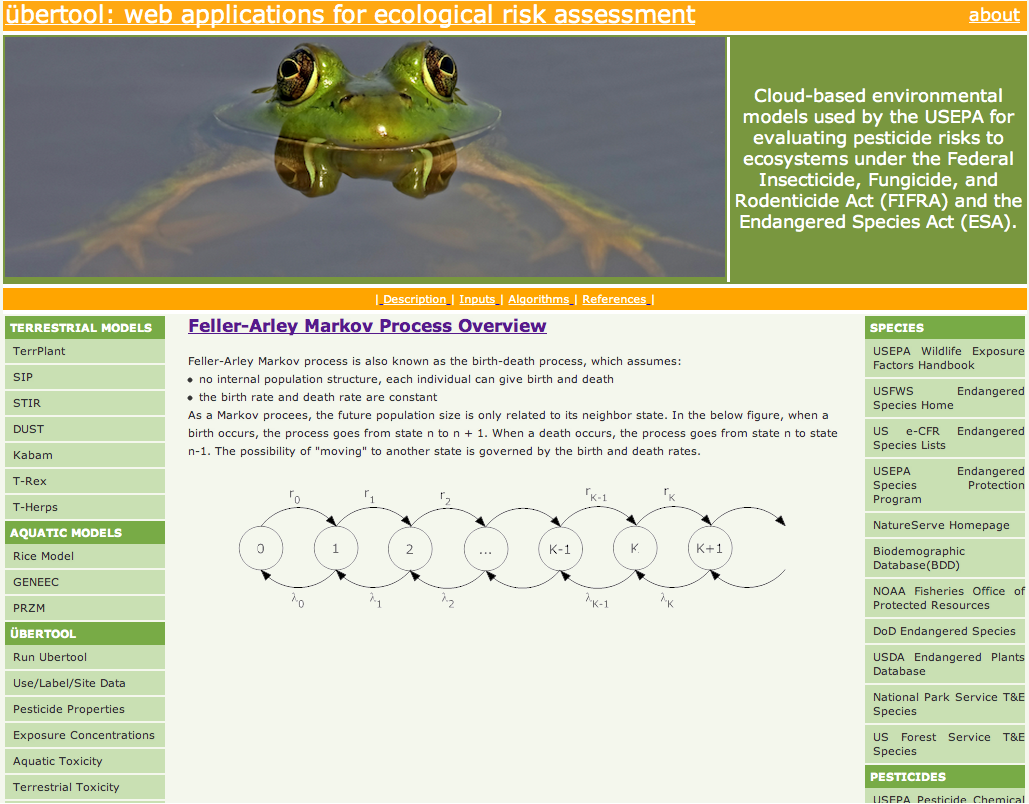
\includegraphics[scale=0.18]{ubertool.png} 
 \caption{\"{u}bertool ecological risk web application}
\end{figure}
\end{frame}

\begin{frame}[fragile]
\frametitle{Getting setup}
\begin{itemize}
  \item{We will use Python 2.7 (not 3)}
  \begin{itemize}
  \item http://www.python.org/getit/
  \end{itemize}
  \item{For Windows users} 
  \begin{itemize}
  \item https://code.google.com/p/pythonxy/wiki/Downloads?tm=2
   \end{itemize}
\end{itemize} 
\end{frame}


\begin{frame}[fragile]
\frametitle{Some extra libraries to install}
\begin{itemize}
  \item{numpy- http://sourceforge.net/projects/numpy/}
\end{itemize} 
\end{frame}

%\begin{frame}[fragile]
%\frametitle{Need a text editor}
%\begin{itemize}
%  \item{Linux}
%  \item{Mac}
%  \begin{itemize}
%  \item TextWrangler
%  \item Smultron
%  \item TextEdit (already installed)
%  \end{itemize}
%  \item{Windows}
%  \begin{itemize}
%  \item Notepad (already installed)
%  \item Notepad++
%  \item TextPad
%  \end{itemize}
%\end{itemize} 
%\end{frame}

\begin{frame}[fragile]
\frametitle{Download the exercise scripts for this class}
\begin{itemize}
  \item \href{http://www.ubertool.org}{http://www.ubertool.org}
  \item Created with Python as the science engine
\end{itemize} 
\end{frame}

\begin{frame}[fragile]
\frametitle{Opening a shell and running Python}
\begin{itemize}
  \item{Mac- Spotlight and type 'terminal'}
  \begin{figure}
 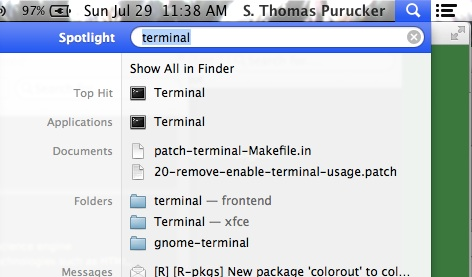
\includegraphics[scale=0.2]{mac_terminal.jpg} 
 \caption{Opening terminal in OS X}
\end{figure}
  \item{Windows- Type 'cmd' in search window for command prompt}
  \begin{figure}
 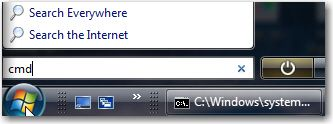
\includegraphics[scale=0.4]{win_cmd.jpg} 
 \caption{Opening the command prompt in Windows 7}
\end{figure}
\end{itemize} 
\end{frame}

\begin{frame}[fragile]
\frametitle{Check Python installation}
\begin{enumerate}
\item Type 'python' at the shell prompt
\item  Then type at the Python prompt:
\begin{lstlisting}
import sys
sys.version
import numpy
numpy.__version__
quit()
\end{lstlisting} 
\end{enumerate}
\end{frame}

\begin{frame}[fragile]
\frametitle{Run a script at the command line}
\begin{lstlisting}
# save this in a text file as hello.py
print "Hello Minneapolis!"
# then navigate to its directory in a shell
# and run at the command prompt with 
# python hello.py
\end{lstlisting}
\end{frame}

\begin{frame}[fragile]
\frametitle{Run IDLE}
\begin{itemize}
  \item IDLE is the "Interactive DeveLopment Environment" bundled with Python
  \item Type 'IDLE' in Mac Spotlight or Windows search window
  \item Or type 'idle' from the python prompt
  \begin{figure}
 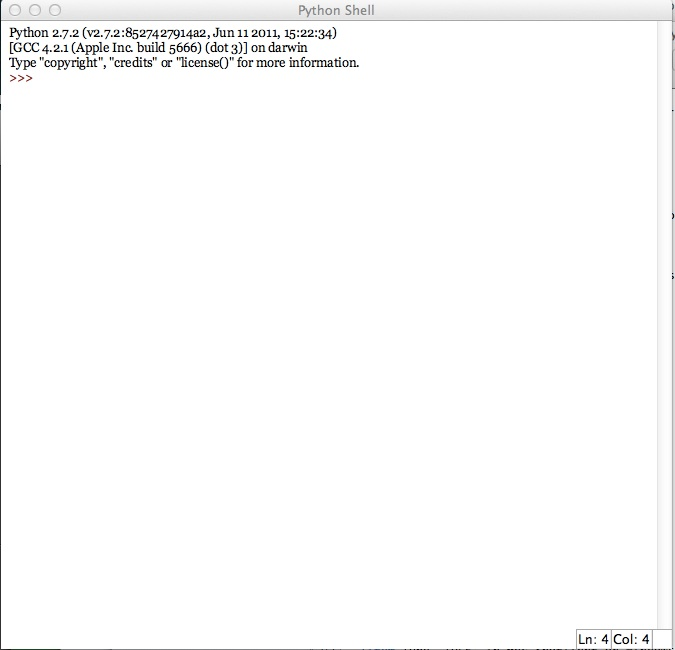
\includegraphics[scale=0.25]{idle.jpg} 
 \caption{IDLE in OS X}
\end{figure}
\end{itemize} 
\end{frame}

\begin{frame}[fragile]
\frametitle{Run hello.py with IDLE}
\begin{enumerate}
\item Open hello.py in scripts directory with File -> Open
\item Run hello.py with Run -> Run Module or (fn) F5
  \begin{figure}
 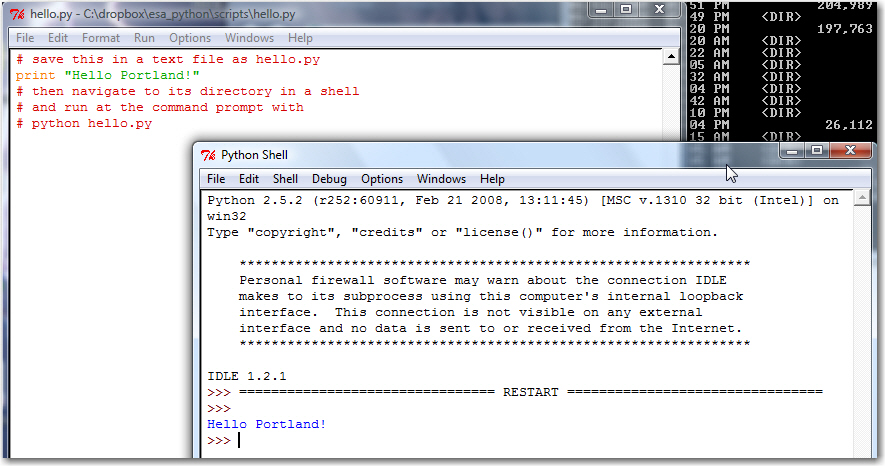
\includegraphics[scale=0.4]{hello_idle.jpg} 
 \caption{Result of running hello.py with IDLE}
 \end{figure}
 \end{enumerate}
\end{frame}

\begin{frame}[fragile]
\frametitle{Variables}
\begin{itemize}
\item No declaration of variables necessary!
\begin{lstlisting}
pop_size = 112 # integer
type(pop_size)
pop_density = 4 # still an integer
type(pop_density)
pop_density = 4. # now its a float
type(pop_density)
species_name = "Oedipina complex" # string
type(species_name)
species_name = "4" # still a string
type(species_name)
\end{lstlisting}
\end{itemize}
\end{frame}

\begin{frame}[fragile]
\frametitle{Basic math operations}
\begin{center}
\begin{tabular}{lc} \hline
\rowcolor{UniBlue!100}Operation & Sign \\ \hline \hline
\rowcolor{UniBlue!75}Addition & + \\ \hline
\rowcolor{UniBlue!90}Subtraction & - \\ \hline
\rowcolor{UniBlue!75}Multiplication & * \\ \hline
\rowcolor{UniBlue!90}Division & / \\ \hline
\rowcolor{UniBlue!75}Power & ** \\ \hline
\rowcolor{UniBlue!90}Modulus & \% \\ \hline
\end{tabular}
\end{center}


\end{frame}

\begin{frame}[fragile]
\frametitle{Be careful about int v float}
\begin{lstlisting}
>>> pop_size = 1086
>>> area = 1254
>>> pop_density = pop_size/area
>>> print(pop_density)
0
>>> type(pop_density)
<type 'int'>
\end{lstlisting}
\begin{alertblock}{Beware}
\begin{itemize}
\item Declare floats by using a decimal point
\item e.g., pop\_size = 1086.
\end{itemize}
\end{alertblock}
\end{frame}

\begin{frame}[fragile]
\frametitle{Python variable naming conventions}
\begin{itemize}
\item all lowercase
\item cannot start with numbers
\item separate\_words\_with\_underscores
\item Style Guide for Python: 
\begin{itemize}
\item http://www.python.org/dev/peps/pep-0008/
\end{itemize}
\end{itemize}
\end{frame}

\begin{frame}[fragile]
\frametitle{unittest exercises}
\begin{itemize}
\item Exercise 1 uses the unittest library so you can type code and test the result yourself  
\begin{enumerate}
  \item Edit the script in IDLE between the \# and the selfassert calls
  \item Run it 
  \item If it complains, fix it and run it again!
\end{enumerate}
\begin{alertblock}{Beware}
\begin{itemize}
\item Python is very picky about space formatting, start your editing right below each \# (8 spaces over)
\item Python is case-sensitive- diffusion\_rate and Diffusion\_rate are different variables
\end{itemize}
\end{alertblock}
\end{itemize}
\end{frame}

\begin{frame}[fragile]
\frametitle{Exercise 1- Run the script exer01\_variables.py}
\Fontix
\begin{lstlisting}
import unittest

class TestVariables(unittest.TestCase):
    def test_variables(self):
        # create the variable `diffusion_rate`, 
        # and assign it a float value of 6.0
        # ********************************************

        self.assertEqual(diffusion_rate, 6.)
        self.assert_(isinstance(diffusion_rate, float))

        # assign ``cohort_size`` to an integer value of 84
        # ********************************************
        
        self.assertEqual(cohort_size, 84)
        self.assert_(isinstance(cohort_size, int))

        # create a variable `species_name`,
        # and assign it to 'Pieza kake'
        # ********************************************

        self.assertEqual(species_name, "Pieza kake")
        self.assertTrue(isinstance(b, str))
        
if __name__ == '__main__':
    unittest.main()
\end{lstlisting}
\end{frame}




%\begin{frame}[fragile]
%\frametitle{Hello world! (from an interpreter)}
%\begin{lstlisting}
%>>> python
%>>> print "Hello world!"
%Hello world!
%\end{lstlisting}
%\end{frame}

%\begin{frame}[fragile]
%\frametitle{Hello world! (from a script)}
%\begin{lstlisting}
%# save this in a text file as hello.py
%print "Hello world!"
%# then run at the command prompt with 'python hello.py'
%\end{lstlisting}
%\end{frame}

%\begin{frame}[fragile]
%\frametitle{Hello world! (as an executable)}
%\begin{lstlisting}
%#!/usr/bin/env python
%# the above line automatically invokes Python
%# save this in a text file as hello_exe.py
%print "Hello world!"
%# we can run this with simply "hello"
%\end{lstlisting}
%\end{frame}

\end{document}